\documentclass{dsadokumentation}

\usepackage{amssymb}
\usepackage{amsthm}
\usepackage{algorithm}
\usepackage[noend]{algpseudocode}
\usepackage{wrapfig}



\addbibresource{kurs2.6.bib}

% set this to your course number minus 1
\setcounter{chapter}{1}

\newcommand\myacademy{Wolfsberg 2022}
% \usepackage{showframe}

\begin{document}

\kurs{Die Theorie der Information}{Wie aus Daten Bilder werden}{example-image-a}

\section{Aus der Kursbeschreibung}
\sectionauthor{Joachim Gomoletz, Jenny Süfke}

Kaum ein Teilgebiet der Algebra hat einen so umfangreichen (auch außermathematischen) Anwendungskreis gefunden wie die Boolesche Algebra.
Ihr Erfinder George Boole (1815--1864) entwickelte 1854 in seinem Buch \enquote{An Investigation of the Laws of Thought} eine \enquote{Algebra der Logik}, in der er durch abstrakte Rechengesetze die philosophische Logik zu einer mathematischen Logik formalisierte.
Anwendungen dieser Theorie finden sich nicht nur in der Technik bei der Konstruktion elektronischer Schaltkreise und künstlicher Intelligenzen, sondern z.B.\ auch in der Maßtheorie und Wahrscheinlichkeitsrechnung.
Die Boolesche Algebra umfasst die Mengen- und Schaltalgebra und ist damit eine wichtige Grundlage in der Mathematik und Technik.
Durch die Konstruktion von logischen Schaltungen bis hin zu ganzen Computern ist sie die entscheidende Basis der Informatik.

Das Erarbeiten eines mathematischen Themas erfordert umfangreiche und detaillierte Kenntnisse der mathematischen Sprache und Arbeitsweise, zu der das Verständnis von mathematischen Begriffen, Symbolen und Konzepten gehören.
Um eine Erarbeitung der Booleschen Algebra auf universitärem Niveau zu gewährleisten, werden zunächst die Grundlagen der Mengenlehre, von Relationen, Quantoren und Aussagen gelegt.
Außerdem werden die elementaren Beweistechniken vorgestellt und in das Arbeiten mit \LaTeX{} eingeführt.
Mittels Vorträgen der Teilnehmenden wird ein Überblick über das Thema Boolesche Algebra gegeben.
Es werden so fundamentale Kenntnisse beispielsweise zu den Themen Aussagenlogik, Schaltalgebra, Boolesche Algebren, Ringe und Verbände erworben.
Als Grundlage für die Vorträge dient der Reader der Technischen Hochschule Darmstadt \enquote{Boolesche Algebra} von Dr.\ Heinz-Peter Gumm und Dr. Werner Poguntke.
Nach diesem ersten Teil des Kurses wird selbständig an Projekten gearbeitet.
In der Projektphase haben die Teilnehmenden die Möglichkeit, sich auf ein Teilgebiet der Algebra einzuschränken und dieses in der Tiefe zu erarbeiten.
Dabei ist die Richtung des Projektes nicht vorgegeben.
Die Teilnehmenden erhalten so die Möglichkeit, in Kleingruppen die kennengelernten Methoden und Konzepte autodidaktisch anzuwenden.
Die Projektthemen reichen von technischen Anwendungen wie dem Halbaddierer über das Arbeiten mit logischen Programmiersprachen (wie z.B.\ Prolog) bis zur Ausarbeitung von Beweisen.
Regelmäßig wird dem Kurs berichtet, wie die Gruppen mit ihren Projekten vorankommen.
Im letzten Kursteil werden die Ergebnisse der Projektarbeit in Form von Vorträgen dem Kurs präsentiert und schriftlich dokumentiert.


\section{Ein Kapitelname}
\sectionauthor{Autorin 1, Autor 2}

Hier folgen ein paar Tipps, wie man \LaTeX{} verwendet.

\begin{itemize}
	\item Wir wollen nun ein Zitat erstellen, dass in Klammern hinter einem Satz erscheint \parencite{k2.6.somelabel}. Und jetzt erzählen wir davon, wie \textcite{k2.6.somelabel} seine Theorie beschreibt.

	\item Anführungsstriche sind mit \LaTeX{} ein bisschen speziell. Deshalb verwenden wir das Paket csquotes. Wenn ihr mehr als simple Anführungsstriche braucht, schaut gerne in der Dokumentation von csquotes im Internet nach. Und so \enquote{mache ich Anführungsstriche}.

	\item So zitiere ich einen längere Block: \textquote[\cite{k2.6.somelabel}]{Ich bin ein langer Text, der gerne zitiert wird. Das Gute an diesem Befehl ist, dass die Zitation hinten automatisch erzeugt wird.}
\end{itemize}

\section{Nächstes Kapitel}\label{k2.6.ch.einkapitel}
\sectionauthor{Autorin 3, Autor 4}

In diesem Kapitel passiert nicht viel, außer dass wir ihm einen Namen geben, damit wir es später referenzieren können.

\section{Und noch eins}
\sectionauthor{Autorin 1, Autor 3}

Die Kolleg*innen haben haben in \cref{k2.6.ch.einkapitel} aber etwas Spannendes geschrieben.
Und wir machen jetzt hier mit einer Tabelle und eine Figur weiter.

Wollen wir eine Tabelle am Anfang eines Satzes referenzieren, machen wir das so. \Cref{k2.6.tab.bestetabelle} ist eine sehr schöne Tabelle. Das großgeschriebene \enquote{Cref}, führt dazu, dass das Wort \enquote{Tabelle} ausgeschrieben wird und wird am Anfang eines Satzes verwendet. Genauso funktioniert es auch mit Referenzen auf Abschnitte. \Cref{k2.6.ch.einkapitel} is ein schöner Abschnitt.

Das kleingeschriebene \enquote{cref} verwendet man innerhalb eines Satzes, wenn man zum Beispiel von \cref{k2.6.ch.einkapitel} spricht.

\begin{table}
	\centering
	\begin{tabular}{lrl}
		\toprule
		Hier           & ist die               & erste Zeile     \\\midrule
		Jetzt          & kommt der Hauptinhalt & der Tabelle     \\
		Und weil es so & schön ist             & noch eine Zeile \\
		\bottomrule
	\end{tabular}
	\caption{Eine schöne Tabellenunterschrift}
	\label{k2.6.tab.bestetabelle}
\end{table}

\section{Ein paar Regeln}
Damit am Ende alle Beiträge gut zusammengefügt werden können, sind ein paar Regeln wichtig.

\begin{figure}
	\centering
	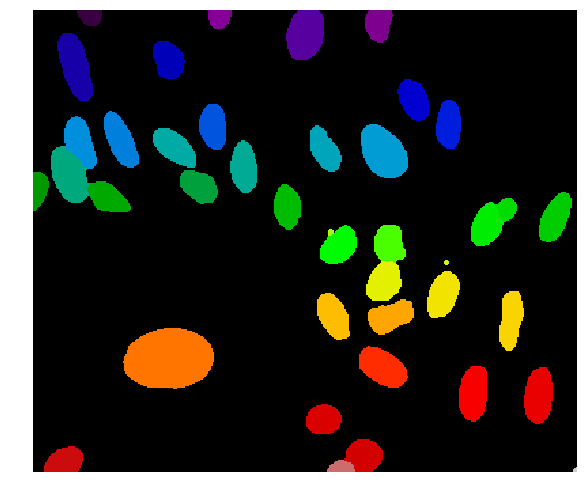
\includegraphics[width=0.5\textwidth]{k2.6/exampleimage.png}
	\caption{Eine richtig gute Abbildung.}
	\label{k2.6.fig.meinefigure}
\end{figure}

\begin{enumerate}
	\item WICHTIG: Alle Namen für Referenzen (also Namen für Bibliografieeinträge, alles wo ihr \enquote{\textbackslash label} oder \enquote{\textbackslash textcite} oder \enquote{\textbackslash parencite} verwendet), muss mit \begin{center} \enquote{k\textit{akademienummer}.\textit{kursnummer}.} \end{center} beginnen.

	\item Für alle Referenzen innerhalb des Dokuments verwenden wir das Paket cleveref (s.u.). Verwendet kein reines \textbackslash ref!
	\item Bei der Verwendung von Figuren und Tabellen ist es wichtig, dass diese unmittelbar vor dem Absatz, in dem sie das erste Mal referenziert wird, auftaucht. Vertraut grundsätzlich darauf, dass \LaTeX{} die Figur oder die Tabelle am Ende an einen guten Ort setzen wird. In fast allen Fällen muss man nicht von Hand machen.
  \item Falls ihr das braucht, dürft ihr gerne weitere \LaTeX{}-Pakete einbinden. Seid aber bitte zurückhaltend und tut dies nur, wenn ihr es wirklich braucht.
		Beispielsweise könnt ihr, wie hier beschrieben \href{https://en.wikibooks.org/wiki/LaTeX/Floats,_Figures_and_Captions#Wrapping_text_around_figures}{(Link)}, mit dem Paket \emph{wrapfigure} Text direkt um eine Abbildung herum fließen lassen.
	\item Bibliographie und Zitate
	      \begin{itemize}
		      \item Wir verwenden biblatex mit biber. Jeder Kurs erstellt eine Bibliographie-Datei, wie in diesem Dokument beispielsweise vorgeführt.
		      \item Für Verweise auf Bibliografieeinträge verwenden wir entweder \enquote{\textbackslash textcite} für Zitate innerhalb eines Satzes und \enquote{\textbackslash parencite} für Zitate, die am Ende eines Satzes stehen.
	      \end{itemize}
\end{enumerate}


Und als allerletztes noch ein paar fortgeschrittene \LaTeX{}-Tipps:
\begin{itemize}
	\item Nach Punkten, die eine Abkürzung anzeigen und keinen Satzabschluss darstellen, muss ein zusätzlicher Backslash eingefügt werden: Dr.\ Heinz-Peter Gumm. Ansonsten ist die Lücke hinter dem Punkt zu groß.
	\item Falls eine Satz mit mehreren Großbuchstaben endet, muss hinter dem Punkt ein \enquote{\textbackslash @} eingefügt werden, damit \LaTeX{} weiß, dass es einen großen Abstand machen muss: Die Weltraumstation heißt ISS.\@ Wir brauchen einen Abstand.
	\item Es gibt verschiedene Zeichen, die alle ungefähr wie ein Bindestrich aussehen: $-$ (Minuszeichen in Formeln), - (Bindestrich), -- (Halbgeviertstrich), --- (Geviertstrich). Die haben alle unterschiedliche Bedeutungen. Wichtig ist, wenn man einen Bereich angeben möchte (zum Beispiel eine Anfangs- und eine End-Jahreszahl), nimmt man nicht \enquote{-} sondern \enquote{--}: 2004--2022.
\end{itemize}

% diese Zeile darf entfernt werden

\printbibliography{}

\end{document}
